\documentclass[main.tex]{subfiles}

\begin{document}

\subsection{Primo esercizio}

 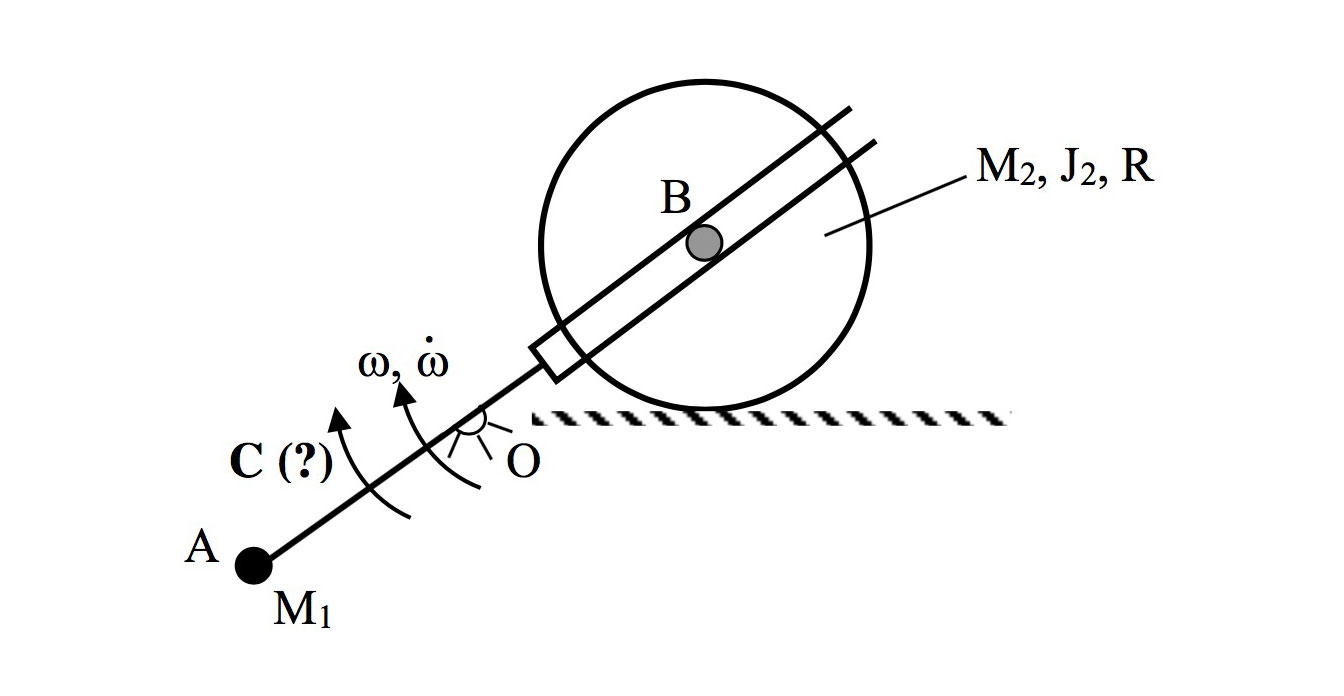
\includegraphics[width=\textwidth]{2015-2207-1.jpg}

\begin{alignat*}{5}
	M_1 = 30\,kg \quad
	M_2 = 20\,kg \quad
	J_2 = 1\,kg m^2 \quad
	R = 0.2\,m
\end{alignat*}
\begin{alignat*}{5}
	OB = 0.4\,m\quad
	AO = 0.3\,m\quad
	\omega = 1\,rad/s\quad
	\dot{\omega}=0.4\,rad/s^2\quad
\end{alignat*}


Il sistema rappresentato in figura è posto nel piano verticale.

Un piolo, rigidamente vincolato al centro B del disco, scorre all’interno del glifo incernierato in O, da considerarsi di massa e momento di inerzia trascurabili. All’estremo A del glifo è vincolata una massa puntiforme $M_1$. Il disco, di massa $M_2$, momento d’inerzia baricentrico $J_2$ e raggio $R$, rotola senza strisciare lungo una guida orizzontale.

Note la velocità angolare $\omega$ e l’accelerazione angolare $\dot{\omega}$ del glifo si chiede di calcolare:

\begin{enumerate}
	\item La velocità angolare e l’accelerazione angolare del disco.
	\item La coppia $C$ necessaria per garantire la condizione di moto assegnata.
\end{enumerate}

\clearpage

\subsection{Soluzione primo esercizio (non corrispondente)}

\paragraph{Osservazioni importanti}

\begin{enumerate}
	\item Il segmento OB, essendo un \textit{glifo}, ha lunghezza variabile.
	\item Il CIR (\textit{centro di istantanea rotazione}) del disco coincide con il punto di contatta sulla superficie.
	\item La \textit{velocità angolare} $\omega$, l'\textit{accelerazione angolare} $\dot{\omega}$ e la \textit{coppia} $C$ ruotano in \textbf{senso orario}.
	\item Il punto B si trova ad una $y_B = R = 0.2\,m$
	\item Il disco non si muove verso l'alto, quindi la sua componente verticale di velocità sarà nulla. Ragionamento analogo può essere fatto per l'accelerazione.
\end{enumerate}

\paragraph{Primo punto}
Procedo con il metodo dei numeri complessi, definendo $b=OB$ e $\alpha$ come l'angolo sotteso all'asta:

\subparagraph{Spostamento}

\begin{align*}
	B &= be^{i\alpha}\\
	B &=  \begin{cases}
		Y_B = R = b\sin\alpha\\
		X_B = b\cos\alpha
	\end{cases}
	\Longrightarrow \begin{cases}
		\alpha = \arcsin(\frac{R}{b}) = \frac{\pi}{6}\,rad\\
		X_B = b\cos\alpha = 0.2\sqrt{3}\,m
	\end{cases}
\end{align*}

\subparagraph{Velocità}
Derivo ed ottengo le velocità:

\begin{align*}
	v_B &= b\dot{\alpha}e^{i(\frac{\pi}{2}+\alpha)} + \dot{b}e^{i\alpha} \\
	v_B &=  \begin{cases}
		v_{y_B} = 0 = b\dot{\alpha}\cos\alpha + \dot{b}\sin\alpha\\
		v_{x_B} = -b\dot{\alpha}\sin\alpha + \dot{b}\cos\alpha\\
	\end{cases}\\
	&= \begin{cases}
		\dot{b} = - \frac{b\dot{\alpha}\cos\alpha}{\sin\alpha} = -b\dot{\alpha}\cot\alpha\\
		v_{x_B} =  -b\dot{\alpha}\sin\alpha - b\dot{\alpha}\cot\alpha\cos\alpha
	\end{cases} \\
	&= \begin{cases}
		\dot{b} = - \frac{b\dot{\alpha}\cos\alpha}{\sin\alpha}\\
		v_{x_B} =  -b\dot{\alpha}(\sin\alpha + \cot\alpha\cos\alpha)
	\end{cases} = \begin{cases}
		\dot{b} = - \frac{b\dot{\alpha}\cos\alpha}{\sin\alpha}\\
		v_{x_B} =  -2b\dot{\alpha}
	\end{cases}\\
\end{align*}
Sostituisco $\dot{\alpha}=-\omega=-1\,rad/s$
\begin{align*}
	\begin{cases}
		\dot{b} = \frac{2\sqrt{3}}{5}\,m/s \\
		v_{x_B} = 0.8\,m/s
	\end{cases}
\end{align*}

Usando gli usuali vincoli cinematici del CIR, procedo a calcolare la velocità angolare del disco:

Ricordando che la velocità risulta essere il \textbf{prodotto vettoriale} di velocità angolare e raggio:
\[
	\vec{v_{x_B}} = \vec{\omega}_{disco}\times\vec{R}
\]
Chiamando $\theta$ l'angolo compreso tra i due vettori, risolvo il \textbf{prodotto vettoriale} come:
\[
	v_{x_B} = \omega_{disco}R\sin\theta
\]

Essendo $\omega_{disco}$ negativo, per la direzione oraria di rotazione del disco, l'angolo che si va a formare tra i due vettore è $\theta=-\frac{pi}{2}$.

\[
	v_{x_B} = \omega_{disco}R\sin(-\frac{pi}{2}) = -\omega_{disco}R
\]

Risolvendo per $\omega_{disco}$ ottengo:

\[
	\omega_{disco} = -\frac{v_{x_B} }{R} = -4\,rad/s
\]

\subparagraph{Accelerazione}
Derivo una seconda volta ed ottengo l'accelerazione:

\[
	a_B =  \dot{b}\dot{\alpha}e^{i(\frac{\pi}{2}+\alpha)} + b\ddot{\alpha}e^{i(\frac{\pi}{2}+\alpha)} - b\dot{\alpha}^2e^{i\alpha} + \ddot{b}e^{i\alpha} + \dot{b}\dot{\alpha}e^{i(\frac{\pi}{2}+\alpha)}
\]

Semplifico l'espressione:

\[
	a_B =  2\dot{b}\dot{\alpha}e^{i(\frac{\pi}{2}+\alpha)} + b\ddot{\alpha}e^{i(\frac{\pi}{2}+\alpha)} - b\dot{\alpha}^2e^{i\alpha} + \ddot{b}e^{i\alpha}
\]

Raccolgo componente normale e tangente:

\[
	a_B =  (2\dot{b}\dot{\alpha} + b\ddot{\alpha})e^{i(\frac{\pi}{2}+\alpha)} +(\ddot{b}- b\dot{\alpha}^2)e^{i\alpha}
\]

Sostituisco $\dot{\alpha} = -\omega = -1\,rad/s$ per semplificare i calcoli:

\[
	a_B =  (-2\dot{b} + b\ddot{\alpha})e^{i(\frac{\pi}{2}+\alpha)} +(\ddot{b}- b)e^{i\alpha}
\]

Separo in componenti cartesiane:
\[
a_B = \begin{cases}
	-(-2\dot{b} + b\ddot{\alpha})\sin\alpha + (\ddot{b}- b)\cos\alpha = a_{x_B}\\
	(-2\dot{b} + b\ddot{\alpha})\cos\alpha + (\ddot{b}- b)\sin\alpha = a_{y_B}
\end{cases}
\]

La componente verticale dell'accelerazione del disco è pari a 0:
\[
a_B = \begin{cases}
	-(-2\dot{b} + b\ddot{\alpha})\sin\alpha + (\ddot{b}- b)\cos\alpha = a_{x_B}\\
	(-2\dot{b} + b\ddot{\alpha})\cos\alpha + (\ddot{b}- b)\sin\alpha = 0
\end{cases}
\]

Ricavo $\ddot{b}$:
\[
	(\ddot{b}- b)\sin\alpha = - (-2\dot{b} + b\ddot{\alpha})\cos\alpha
\]

\[
	\ddot{b} = b - (-2\dot{b} + b\ddot{\alpha})\cot\alpha
\]

Ricavo $a_{x_B}$:
\[
	-(-2\dot{b} + b\ddot{\alpha})\sin\alpha + (b - (2\dot{b} + b\ddot{\alpha})\cot\alpha - b)\cos\alpha = a_{x_B}
\]
\[
	-(-2\dot{b} + b\ddot{\alpha})\sin\alpha - (2\dot{b} + b\ddot{\alpha})\cot\alpha\cos\alpha = a_{x_B}
\]
\[
	-(-2\dot{b} + b\ddot{\alpha})(\sin\alpha +\cot\alpha\cos\alpha) = a_{x_B}
\]
\[
	-2(-2\dot{b} + b\ddot{\alpha}) = a_{x_B}
\]

Sostituisco $\ddot{\alpha}=-\dot{\omega} = -0.4\,rad/s^2$:
\[
	-2(-2\dot{b} - b\dot{\omega}) = a_{x_B}
\]

\[
	2(2\dot{b} + b\dot{\omega}) = a_{x_B}
\]

\[
	2(\frac{4\sqrt{3}}{5} + \frac{4}{25}) = a_{x_B}
\]

\[
	a_{x_B} \approx 3.1\,m/s^2
\]

Utilizzando il legame cinematico dell'accelerazione angolare ottengo:

\[
	\omega_D = \frac{a_{x_B} }{R}\sin(-\frac{\pi}{2}) = -15.5\,m/s^2
\]

\paragraph{Secondo punto}

Per calcolare la coppia $C$ vado ad utilizzare \textit{l'equazione del bilancio delle potenze} (formula \ref{bilancio_potenze_2207}):

\begin{figure}[H]
	\[
		\sum_{i=0}^n W_i = \frac{dE_c}{dt}
	\]
	\caption{Bilancio delle potenze}
	\label{bilancio_potenze_2207}
\end{figure}

\subparagraph{Energia cinetica totale:} prendo in considerazione tutte le masse in movimento ed i loro momenti d'inerzia per poter utilizzare il \textit{teorema dell'energia cinetica}.

\begin{enumerate}
	\item La massa puntiforme $m_1$ si muove di una velocità $v_A = AO\omega$ e non ha momento di inerzia.
	\item La massa del cerchio $M_2$ si muove con una velocità baricentrica calcolata precedentemente come $v_B = 2OB\omega$ e possiede un momento di inerzia baricentrico noto $J_2$.
\end{enumerate}

\[
	E_c = \frac{1}{2}m_1v_A^2 + \frac{1}{2}M_2v_B^2 + \frac{1}{2}J_2\omega_B^2
\]

Sostituisco con i legami cinematici noti ed ottengo:

\[
	E_c = \frac{1}{2}m_1(AO\omega)^2 + \frac{1}{2}M_2(2OB\omega)^2 + \frac{1}{2}J_2(\frac{2OB\omega}{R})^2
\]

Sostituisco nell'equazione $AO = a$ e $OB = b$:

\[
	E_c = \frac{1}{2}m_1(a\omega)^2 + \frac{1}{2}M_2(2b\omega)^2 + \frac{1}{2}J_2(\frac{2b\omega}{R})^2
\]

Raccolgo i coefficienti di $b$ e $\omega$:

\[
	E_c = \omega^2\frac{1}{2}m_1a^2 + 2\omega^2b^2(M_2 + J_2(\frac{1}{R})^2)
\]

Derivo l'equazione, tenendo a mente che i termini che variano nel tempo sono $\omega$ e $b$:

\[
	\frac{E_c}{dt} =  2\omega\dot{\omega}\frac{1}{2}m_1a^2 + 4\omega\dot{\omega}b^2(M_2 + J_2(\frac{1}{R})^2) + 4\omega^2b\dot{b}(M_2 + J_2(\frac{1}{R})^2)
\]

\[
	\frac{E_c}{dt} =  \omega\dot{\omega}m_1a^2 + 4\omega\dot{\omega}b^2(M_2 + J_2(\frac{1}{R})^2) + 4\omega^2b\dot{b}(M_2 + J_2(\frac{1}{R})^2)
\]

\[
	\frac{E_c}{dt} =  \omega(\dot{\omega}m_1a^2 + 4\dot{\omega}b^2(M_2 + J_2(\frac{1}{R})^2) + 4\omega b\dot{b}(M_2 + J_2(\frac{1}{R})^2))
\]

\[
	\frac{E_c}{dt} =  \omega(\dot{\omega}m_1a^2 + 4b(M_2 + J_2(\frac{1}{R})^2)(\dot{\omega}b + \omega \dot{b}))
\]

\subparagraph{La potenza totale:} prendo in considerazione tutte le forze che agiscono sui corpi, eventuali attriti, forze peso e coppie.

\begin{enumerate}
	\item Sul disco agisce una forza peso, contro bilanciata da una forza normale, per cui si annullano reciprocamente. Il disco non subisce l'effetto di attrito volvente o di attriti dinamici.
	\item Sulla massa M1 agisce una forza peso $F_{g_A}$ che non è contro bilanciata da nessuna forza normale.
	\item La coppia $C$ da identificare.
\end{enumerate}

\[
	\sum W_i = \vec{C}\bullet\vec{\omega} + \vec{F}_{g_A}\bullet{\vec{v}_A}
\]

Sostituisco i legami cinematici, con $a = OA$:

\[
	\sum W_i = \vec{C}\bullet\vec{\omega} + \vec{F}_{g_A}\bullet(a\vec{\omega})
\]

Risolvo il prodotto scalare:

\begin{enumerate}
	\item La velocità $\vec{v}_A$ ha una direzione tangente alla circonferenza di raggio $a$ e con verso a $\alpha + \frac{\pi}{2}$. Tra il vettore $\vec{v}_A$ e $\vec{F}_{g_A}$ l'angolo è di $\pi - \alpha$.
	\item La coppia $C$ e la velocità angolare $\omega$ sono concordi, come da testo.
\end{enumerate}

\[
	\sum W_i = C\omega + F_{g_A}a\omega\cos(\pi - \alpha) = C\omega - F_{g_A}a\omega\cos\alpha = \omega(C - m_1ga\cos\alpha)
\]

\subparagraph{Bilancio delle potenze}

\[
	\omega(C - m_1ga\cos\alpha) = \omega(\dot{\omega}m_1a^2 + 4b(M_2 + J_2(\frac{1}{R})^2)(\dot{\omega}b + \omega \dot{b}))
\]

Semplifico $\omega$:

\[
	C - m_1ga\cos\alpha= \dot{\omega}m_1a^2 + 4b(M_2 + J_2(\frac{1}{R})^2)(\dot{\omega}b + \omega \dot{b})
\]

Risolvo per $C$:

\[
	C = m_1ga\cos\alpha + \dot{\omega}m_1a^2 + 4b(M_2 + J_2(\frac{1}{R})^2)(\dot{\omega}b + \omega \dot{b})
\]

Sostituisco numericamente:

\[
	C = 138.9\,Nm\quad(C_{riportato} = 120.2N)
\]

\textbf{Il secondo punto sembra essere errato, non riesco ad identificare l'errore.}


\end{document}